\chapter{Resultados e Discussões}

\section{Resultados para $ F_0 $}\label{sec_F_0}
\subsection{Adaptação do filtro}

Os resultados da adaptação do filtro para uma força $F_0(t) = A_0 sin(2\pi f_0 t)$ com $ N=1000 $  e $ SNR = 90 $ são mostrados na \cref{fig:F0_1000_90_conv}. O número de coeficientes do filtro ($ N_c $) e o fator de convergência ($ \mu $) utilizados são apresentados na figura.

\begin{figure}[!h]
	\centering
	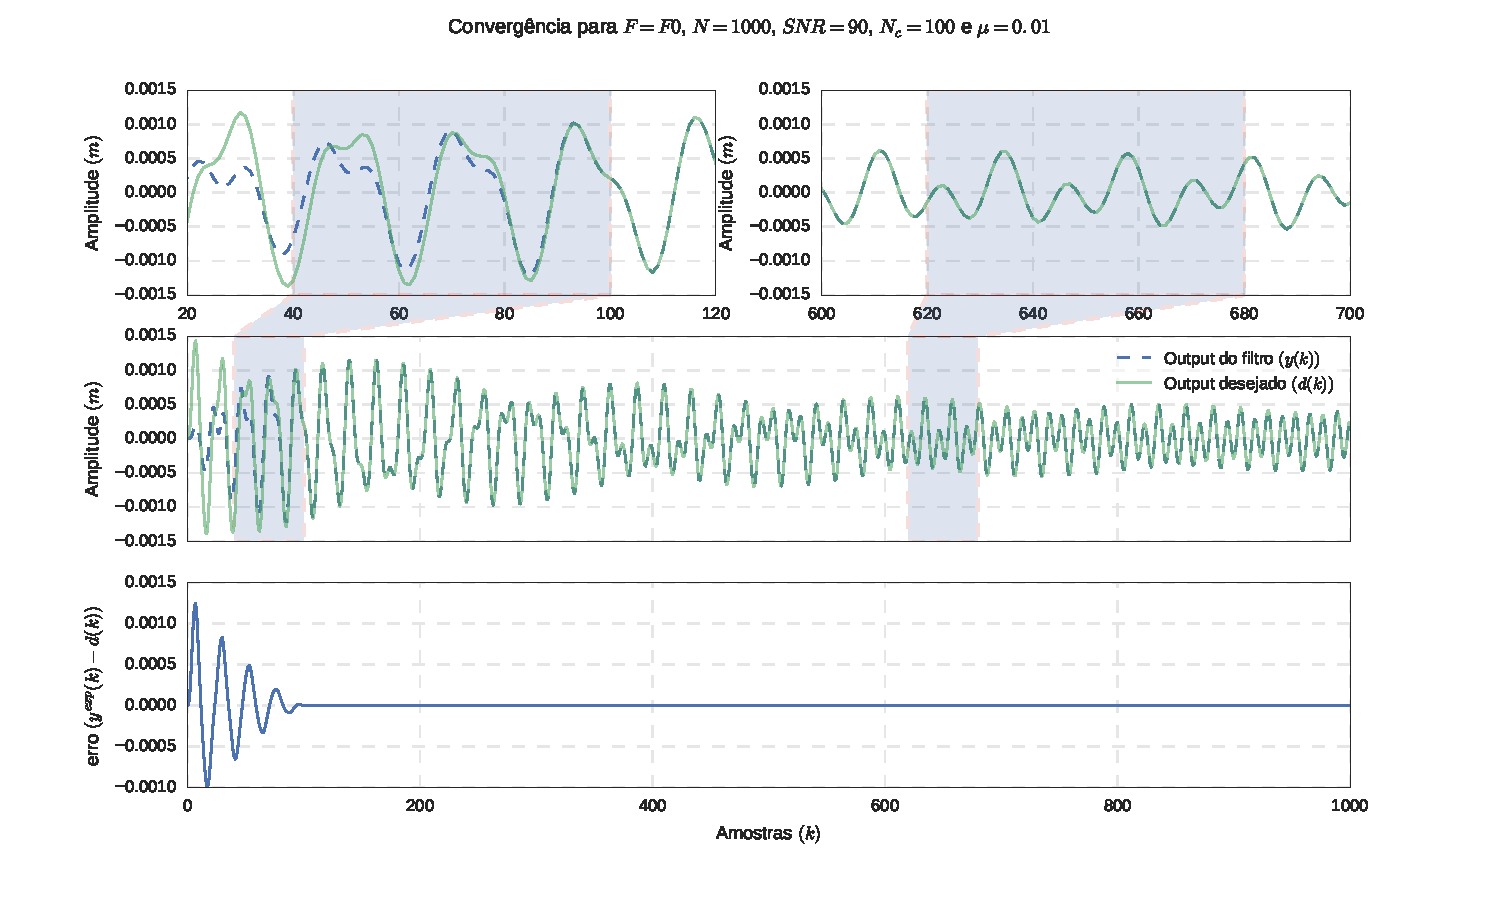
\includegraphics[scale=0.7]{F0_1000_90_conv}
	\caption{Evolução do filtro para $ F=F_0 $, $ N=1000 $ e $ SNR=90 $.}
	\label{fig:F0_1000_90_conv}
\end{figure}

Para o caso do seno puro podemos o filtro tem uma convergência rápida e com menos de 100 iterações o erro já é próximo de zero. 

Na \cref{fig:F0_1000_10_conv} são apresentados os resultados para $ N=1000 $ e $ SNR=10 $. Podemos observar que, mesmo com um nível de ruído mais elevado, o algoritmo apresentou uma convergência rápida.

\begin{figure}
	\centering
	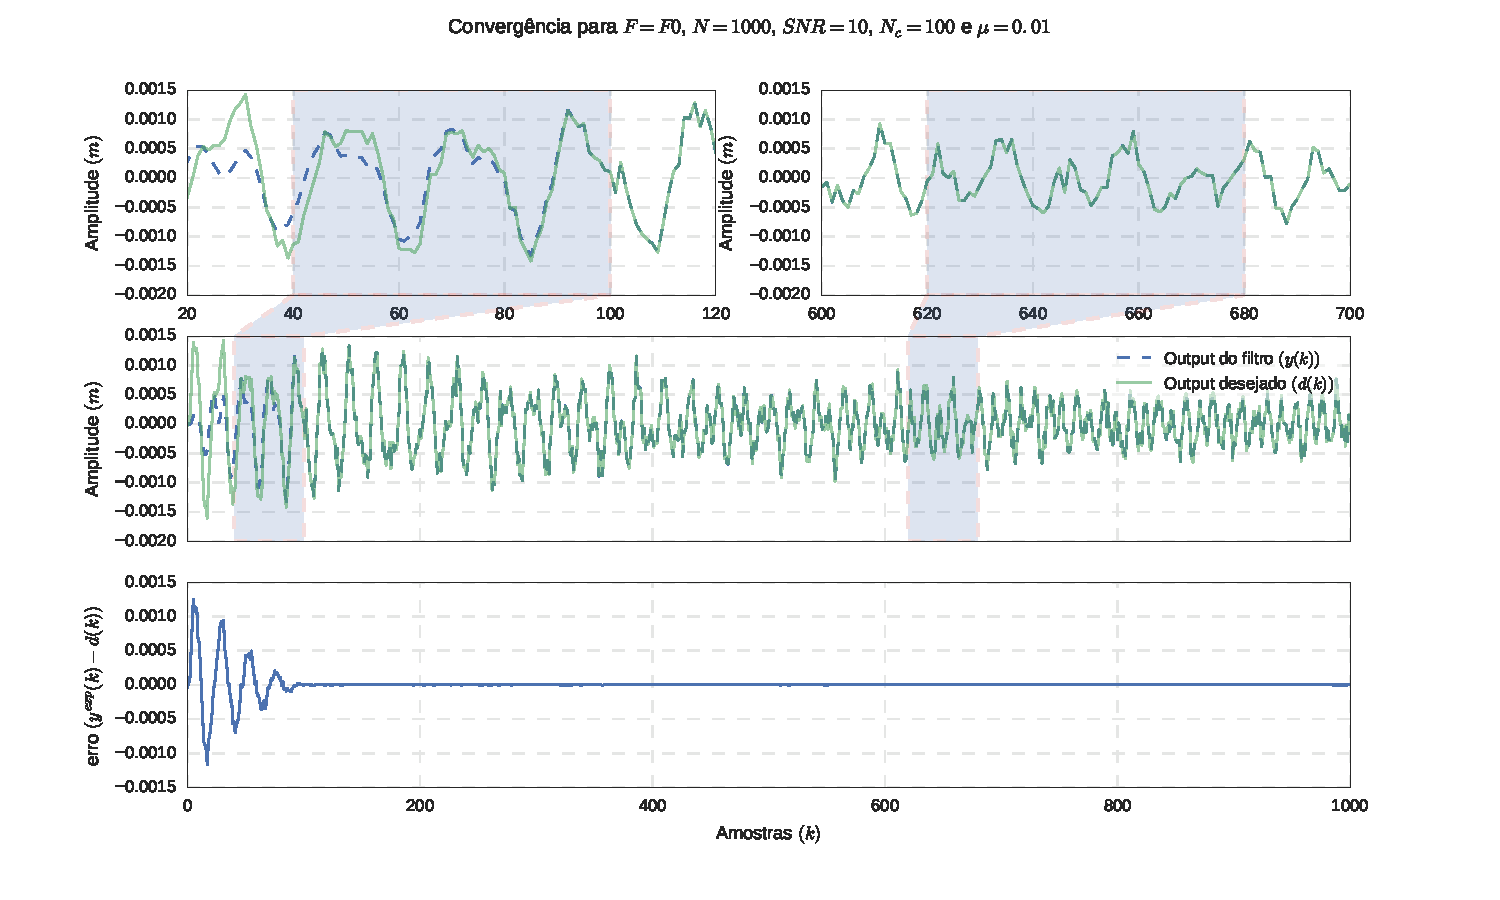
\includegraphics[scale=0.7]{F0_1000_10_conv}
	\caption{Evolução do filtro para $ F=F_0 $, $ N=1000 $ e $ SNR=10 $.}
	\label{fig:F0_1000_10_conv}
\end{figure}

\subsection{FRF do filtro}

Na \cref{fig:F0_1000_90_FRF_med_False} é apresentada a FRF do filtro obtido com $ SNR=90 $ considerando o último vetor de coeficientes, e na \cref{fig:F0_1000_90_FRF_med_True} é apresentada a FRF considerando o vetor obtido através do valor esperado dos coeficientes tomando por base as observações da segunda metade do vetor de dados. A \cref{fig:F0_1000_10_FRF} apresenta os resultados para $ SNR=10 $. 

Podemos observar que FRF do filtro obtido não apresenta bons resultados, aproximando-se do valor esperado apenas na frequência de excitação (\SI{34}{\radian \per \s}). Podemos notar um aumento na amplitude próxima à primeira frequência natural do sistema, mas o valor não se aproxima do esperado. Outro ponto importante é que, para este caso, a FRF do filtro não se mostrou sensível ao nível de ruído. A utilização do último vetor de coeficientes $ w $ ou do valor esperado para a segunda metade do vetor de dados também não teve impacto significativo na resposta. 

\begin{figure}
	\centering
	\begin{subfigure}{0.9\textwidth}
		\centering
		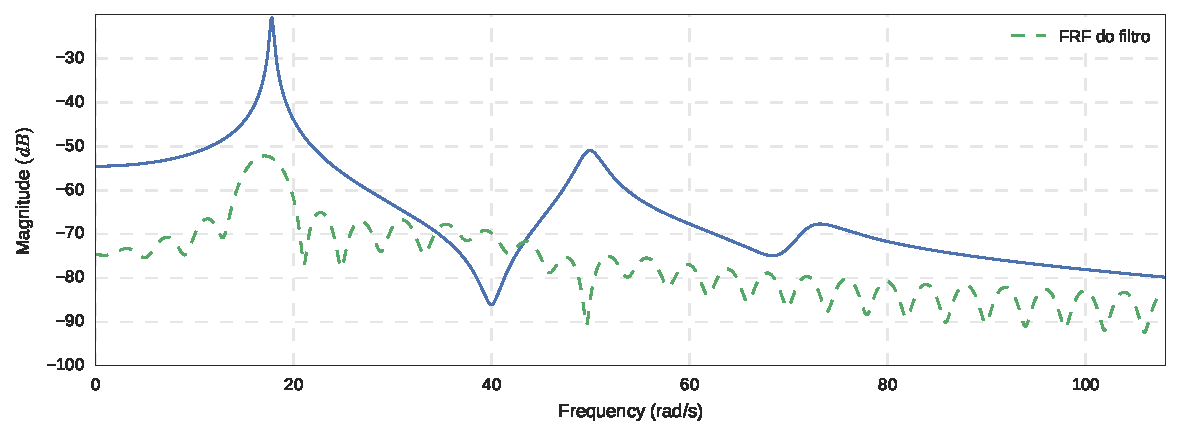
\includegraphics[width=0.9\linewidth]{F0_1000_90_FRF_med_False}
		\caption{último vetor $ w $}
		\label{fig:F0_1000_90_FRF_med_False}
	\end{subfigure}
	\begin{subfigure}{0.9\textwidth}
		\centering
		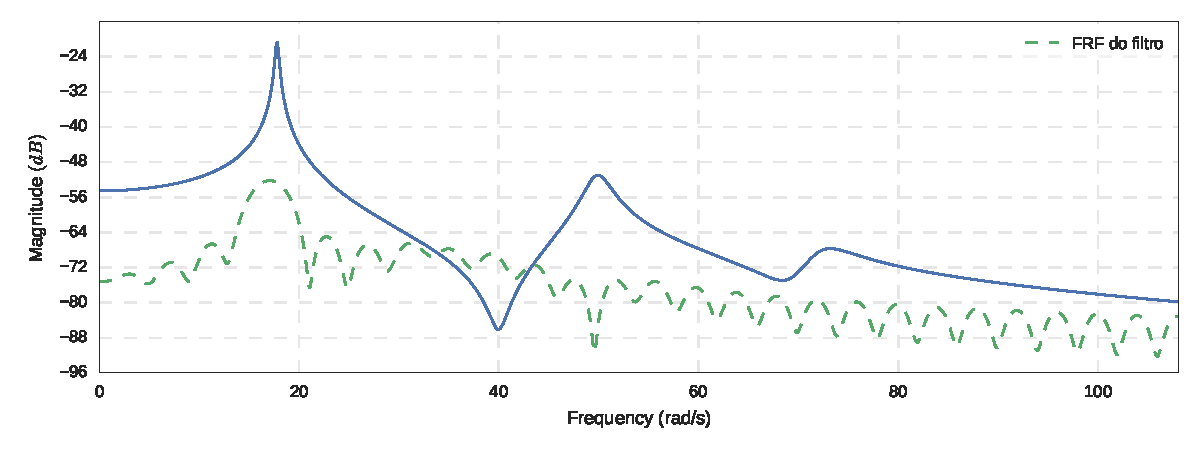
\includegraphics[width=0.9\linewidth]{F0_1000_90_FRF_med_True}
		\caption{valor médio de $ w $}
		\label{fig:F0_1000_90_FRF_med_True}
	\end{subfigure}
	\caption{FRF do filtro obtido para $ F=F_0 $, $ N=1000 $ e $ SNR=90 $.}
\end{figure}

\begin{figure}
	\centering
	\begin{subfigure}{0.9\textwidth}
		\centering
		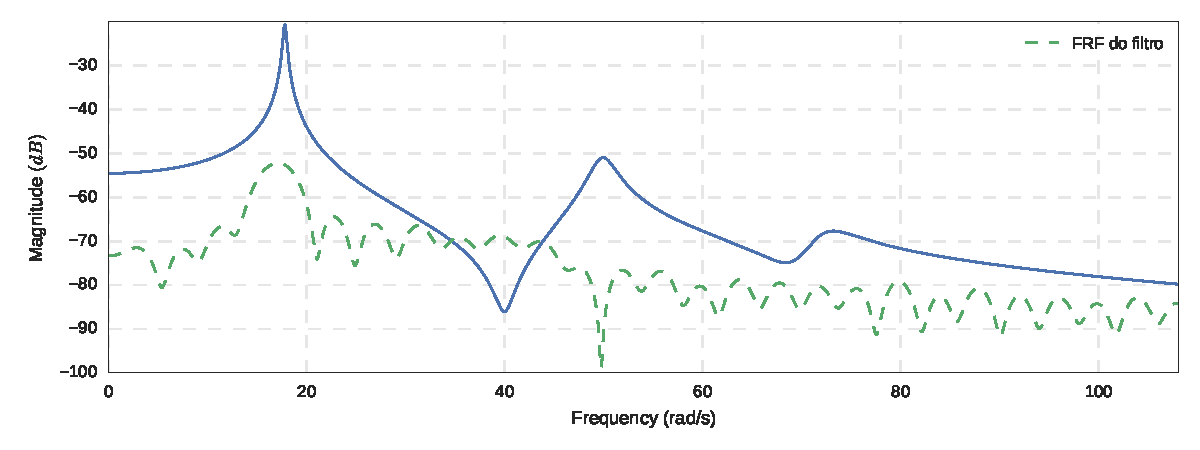
\includegraphics[width=0.9\linewidth]{F0_1000_10_FRF_med_False}
		\caption{último vetor $ w $}
		\label{fig:F0_1000_10_FRF_med_False}
	\end{subfigure}
	\begin{subfigure}{0.9\textwidth}
		\centering
		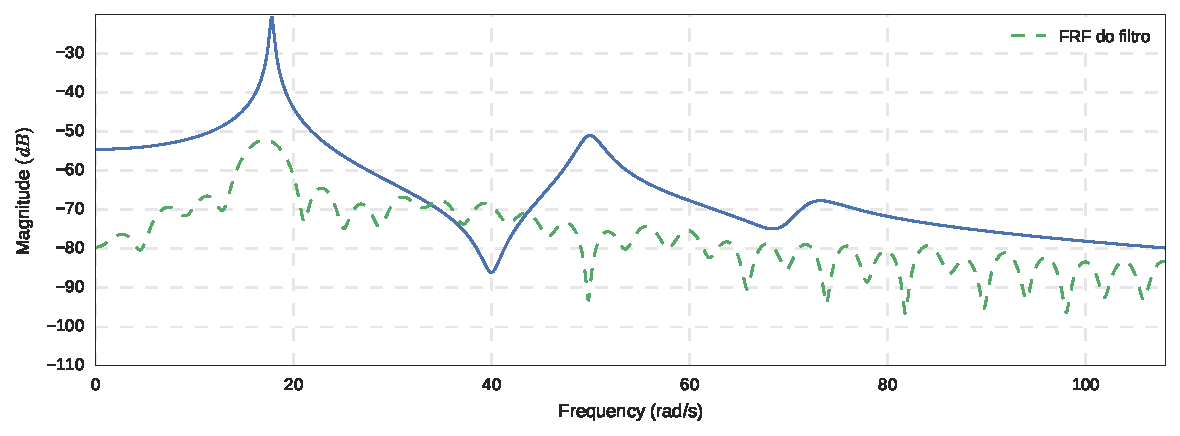
\includegraphics[width=0.9\linewidth]{F0_1000_10_FRF_med_True}
		\caption{valor médio de $ w $}
		\label{fig:F0_1000_10_FRF_med_True}
	\end{subfigure}
	\caption{FRF do filtro obtido para $ F=F_0 $, $ N=1000 $ e $ SNR=10 $.}
	\label{fig:F0_1000_10_FRF}
\end{figure}

\subsection{Predição}

Para analisarmos a predição do filtro, foi escolhida uma força arbitrária $ F_3 $ conforme \cref{eq:F_3}

\begin{equation}\label{eq:F_3}
F_3 = B_1 sin(\omega_1 t)
+ B_2 sin(\omega_2 t)
+ B_3 sin(\omega_3 t)
+ \nu
\end{equation}
onde $ B_1=\SI{1}{\N} $, $ B_2=\SI{2}{\N}$ , $ B_3=\SI{3}{\N} $, $ \omega_1= \SI{14}{\radian \per \s} $, $ \omega_2= \SI{40}{\radian \per \s} $, $ \omega_3= \SI{65}{\radian \per \s} $ e $ \nu $ é um ruído branco de variância 1.

A \cref{fig:F0_1000_90_pred} mostra a predição para o filtro obtido com $ F=F_0 $, $ N=1000 $ e $ SNR=90 $. Podemos observar que a predição obtida com o filtro não é boa e o erro ($ e(n)=y^{exp}(n) - y(n) $) é da ordem do valor previsto pelo filtro.

\begin{figure}[h]
	\centering
	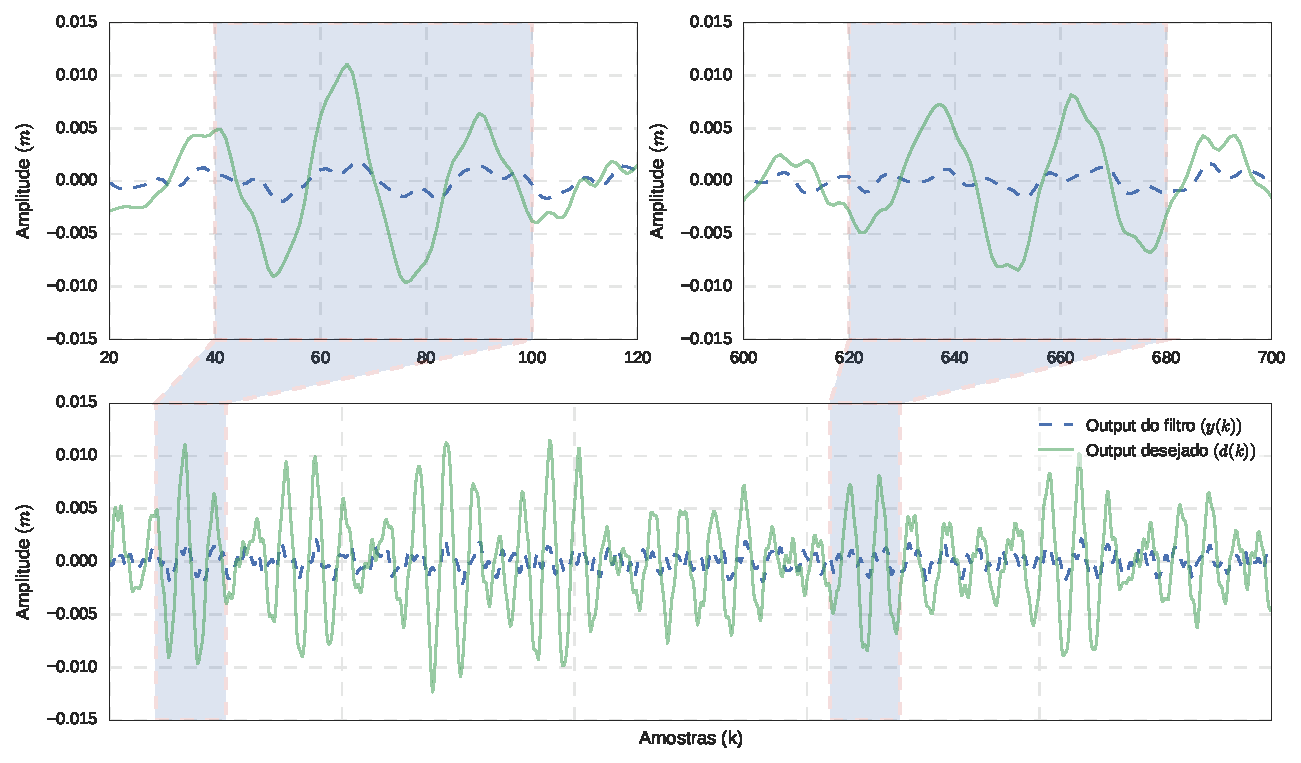
\includegraphics[scale=0.7]{F0_1000_90_pred}
	\caption{Predição do filtro obtido com $ F=F_0 $, $ N=1000 $ e $ SNR=90 $.}
	\label{fig:F0_1000_90_pred}
\end{figure}

Os resultados obtidos para os diferentes valores de $ N $ e $ SNR $ não apresentam diferença para o caso em que $ F=F_0 $ e por isso serão omitidos.

\section{Resultados para $ F_1 $}
\subsection{Adaptação do filtro}

Os resultados da adaptação do filtro para uma força $F_1(t) = A_1 sin(2\pi f_1 t) + A_2 sin(2\pi f_2 t)$  com $ N=1000 $  e $ SNR = 90 $ são mostrados na \cref{fig:F1_1000_90_conv}. Para este caso a convergência se mostrou próxima ao que foi obtido na análise de $ F_0 $. 

\begin{figure}
	\centering
	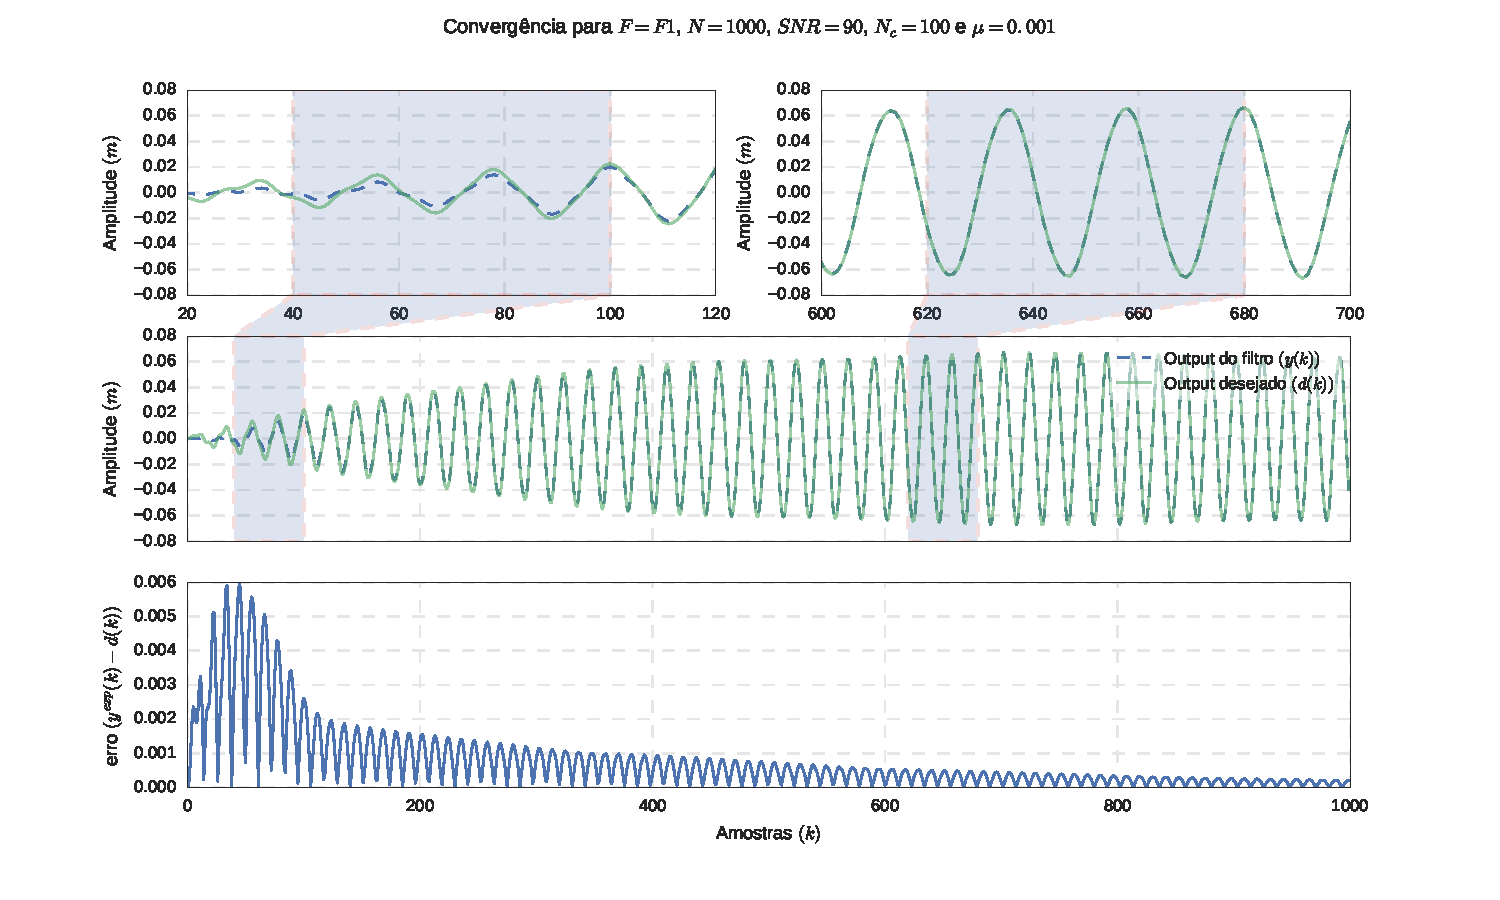
\includegraphics[scale=0.7]{F1_1000_90_conv}
	\caption{Evolução do filtro para $ F=F_1 $, $ N=1000 $ e $ SNR=90 $.}
	\label{fig:F1_1000_90_conv}
\end{figure}

Na \cref{fig:F1_1000_10_conv} são apresentados os resultados para $ N=1000 $ e $ SNR=10 $. Para este caso a convergência não é boa e ao fim das iterações o erro do filtro ainda é alto. 

\begin{figure}
	\centering
	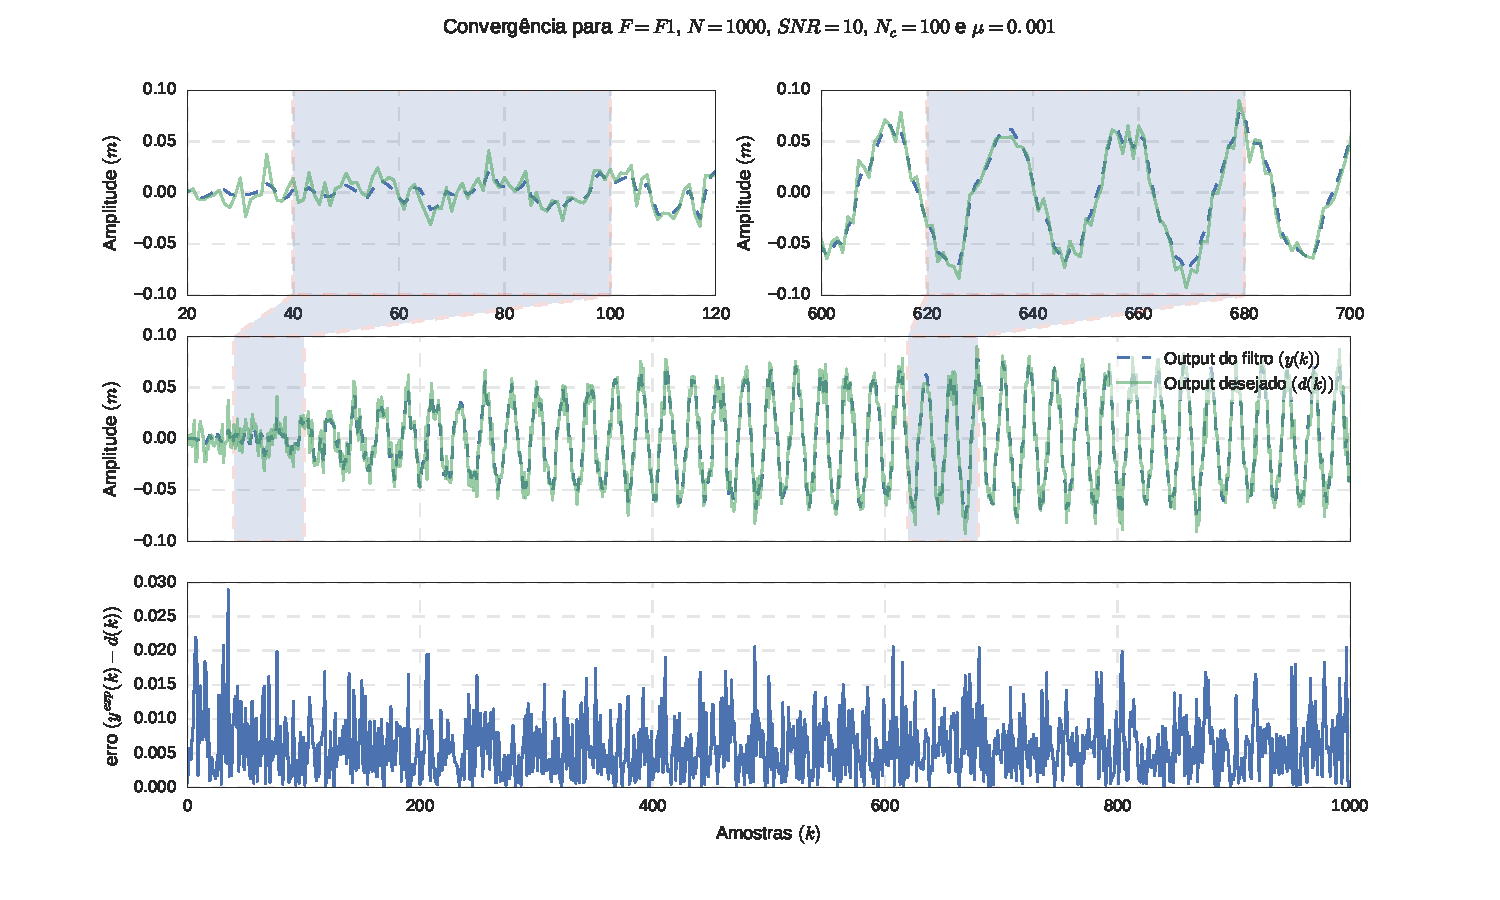
\includegraphics[scale=0.7]{F1_1000_10_conv}
	\caption{Evolução do filtro para $ F=F_1 $, $ N=1000 $ e $ SNR=10 $.}
	\label{fig:F1_1000_10_conv}
\end{figure}

Podemos tentar melhorar a adaptação aumentando o valor do fator de convergência de $ \mu=0.001 $ para $ \mu=0.003 $ o que por sua vez deve aumentar a velocidade de convergência do algoritmo. A \cref{fig:F1_1000_10_mu_003_conv} mostra que, quando utilizamos $ \mu = 0.003 $, o valor de saída do filtro tende a variar mais rapidamente tentando acompanhar o valor desejado, no entanto, as variações bruscas nos valores dos coeficientes do filtro não permitem a convergência e consequente minimização do erro após decorridas várias iterações. 

Conforme \citet{diniz1997adaptive}, o valor de $ \mu $ deve ser escolhido no intervalo mostrado na \cref{eq:mu}

\begin{equation}\label{eq:mu}
0 < \mu < \frac{1}{\lambda_{max}}
\end{equation}
onde $ \lambda_{max} $ corresponde ao maior autovalor da matriz $ {\bf R} $ definida na \cref{eq:mse2}. Podemos concluir que o valor $ \mu = 0.003 $ se encontra fora desse intervalo, já que a convergência não foi atingida e os resultados se apresentaram piores do que os obtidos com $ \mu=0.001 $. 

\begin{figure}
	\centering
	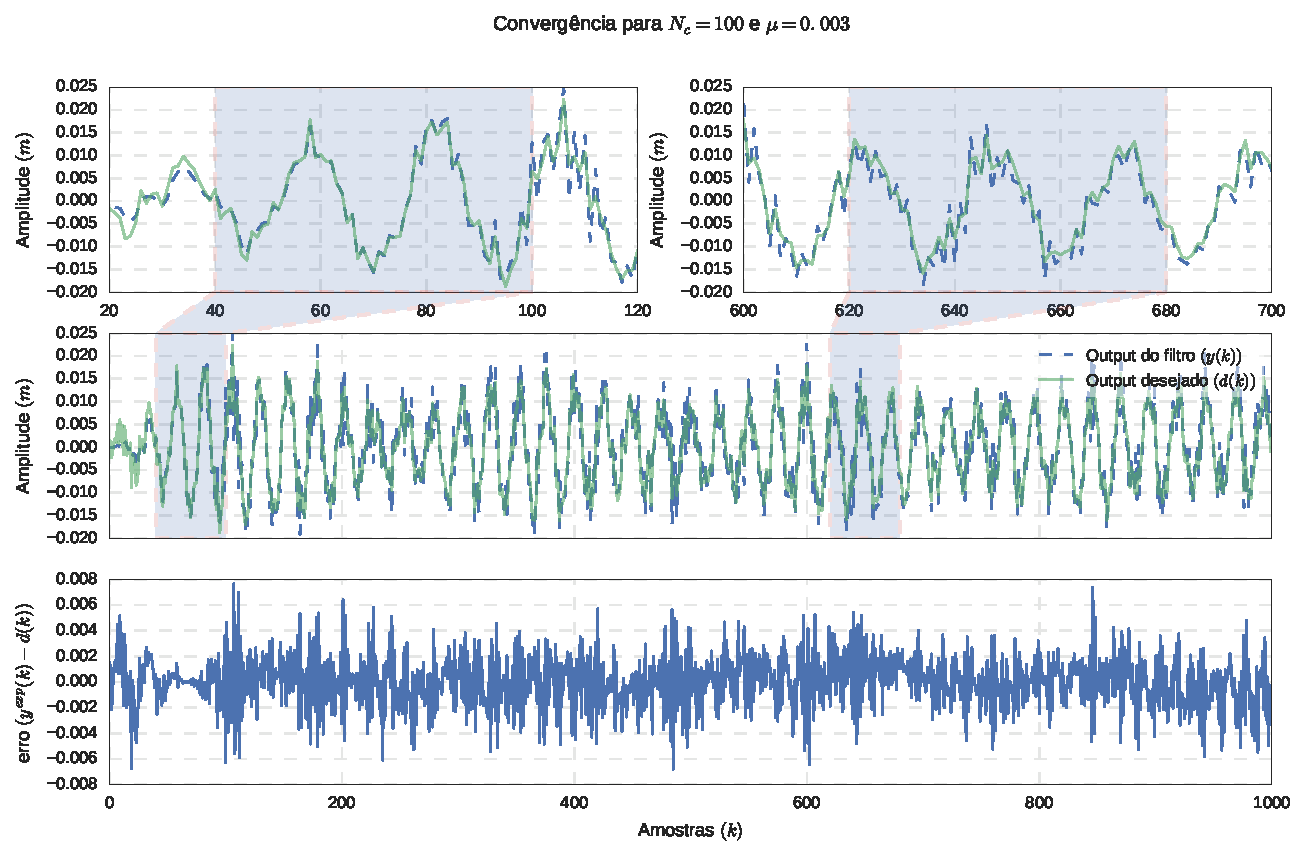
\includegraphics[scale=0.7]{F1_1000_10_mu_003_conv}
	\caption{Evolução do filtro para $ F=F_1 $, $ N=1000 $ e $ SNR=10 $.}
	\label{fig:F1_1000_10_mu_003_conv}
\end{figure}

Para que possamos obter melhores resultados iremos utiliza um fator maior que $ \mu=0.001 $ com o objetivo de aumentar a velocidade de adaptação do filtro e menor que $ \mu=0.003 $ para que a convergência possa ser obtida. A \cref{fig:F1_1000_10_mu_002_conv} mostra que para $ \mu=0.002 $ o filtro atinge a convergência rapidamente, apresentando valores de erro próximos de 0 após 100 iterações.

\begin{figure}
	\centering
	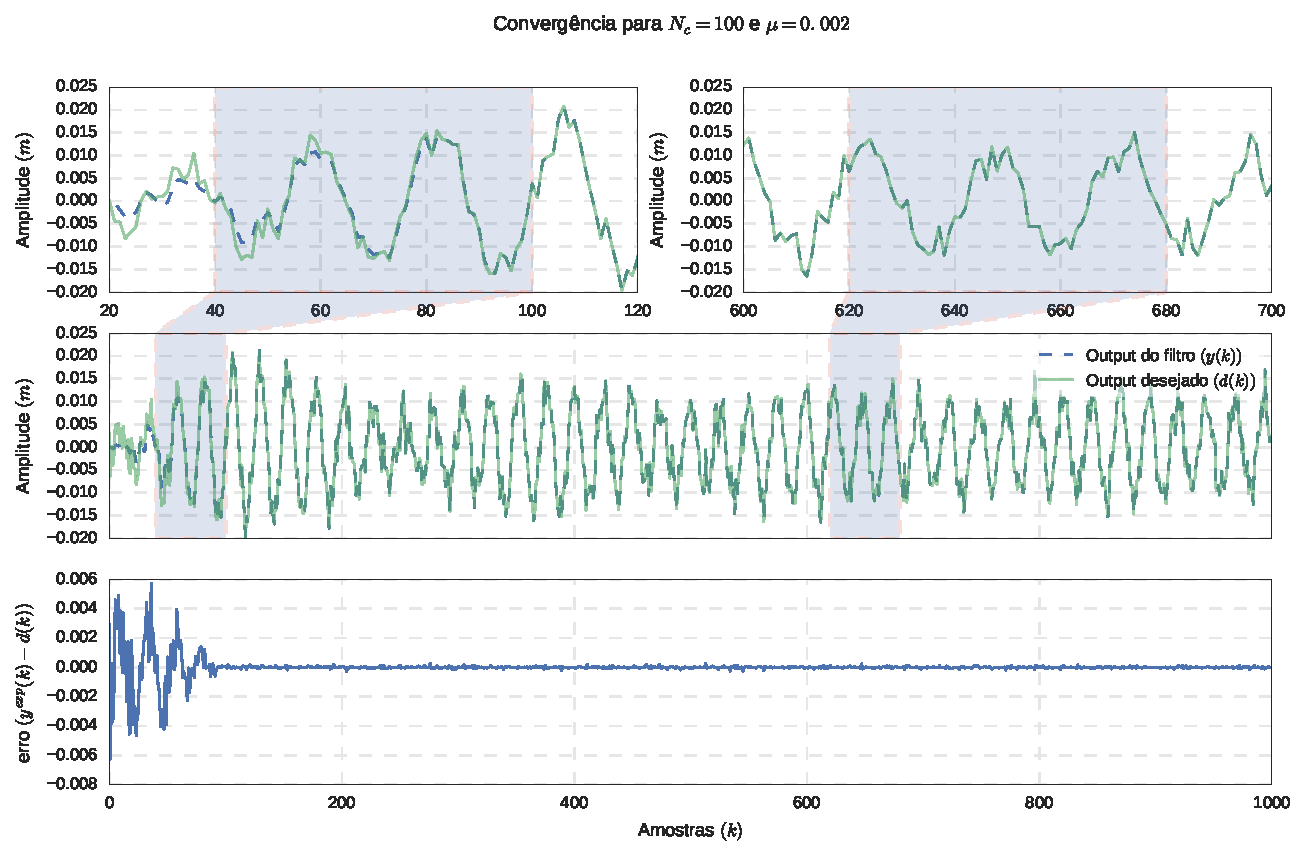
\includegraphics[scale=0.7]{F1_1000_10_mu_002_conv}
	\caption{Evolução do filtro para $ F=F_1 $, $ N=1000 $ e $ SNR=10 $.}
	\label{fig:F1_1000_10_mu_002_conv}
\end{figure}

\subsection{FRF do filtro}
Assim como visto em \ref{sec_F_0}, os resultados para as FRFs se mostraram muito parecidos utilizando-se o último vetor de coeficientes ou o valor esperado dos coeficientes tomando por base as observações da segunda metade do vetor de dados. Sendo assim, iremos apresentar a FRF apenas para o último vetor de coeficientes do filtro.

A \cref{fig:F1_1000_10_mu_002_FRF_med_False} mostra os resultados obtidos com $ N=1000 $ e $ SNR=90 $. Podemos notar uma melhora dos resultados quando comparamos com a FRF obtida para $ F=F_0 $, mas os valores ainda estão distantes da FRF real do sistema.

\begin{figure}
	\centering
	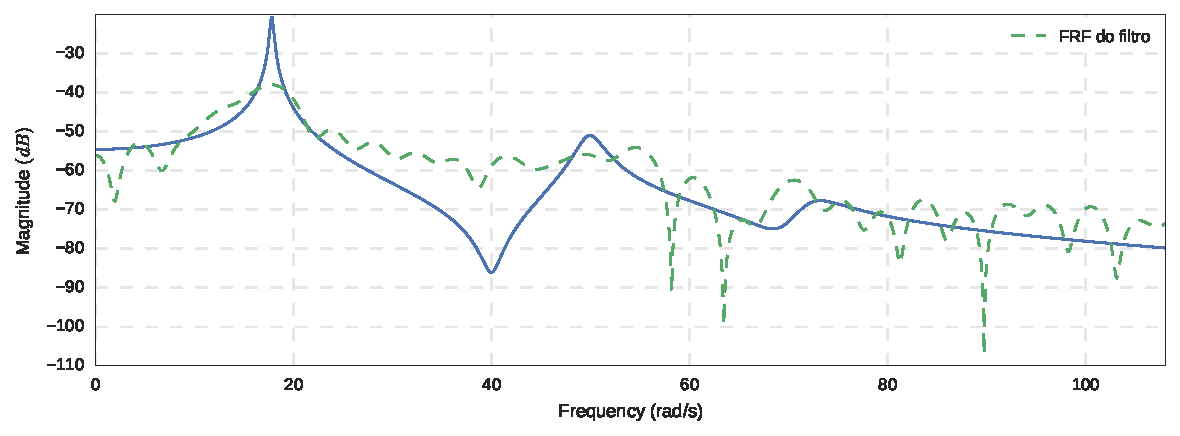
\includegraphics[scale=0.7]{F1_1000_10_mu_002_FRF_med_False}
	\caption{FRF do filtro obtido para $ F=F_1 $, $ N=1000 $ e $ SNR=10 $.}
	\label{fig:F1_1000_10_mu_002_FRF_med_False}
\end{figure}

\subsection{Predição}

Para a predição iremos utilizar a mesma força utilizada em $ F=F_0 $ e descrita na \ref{eq:F_3}. Os resultados da predição são apresentados na \cref{fig:F1_1000_10_mu_002_pred} e mostram uma melhora, mas podemos ver que este filtro também não foi capaz de prever de maneira precisa o comportamento do sistema para uma força diferente da utilizada no processo de adaptação.

\begin{figure}[h]
	\centering
	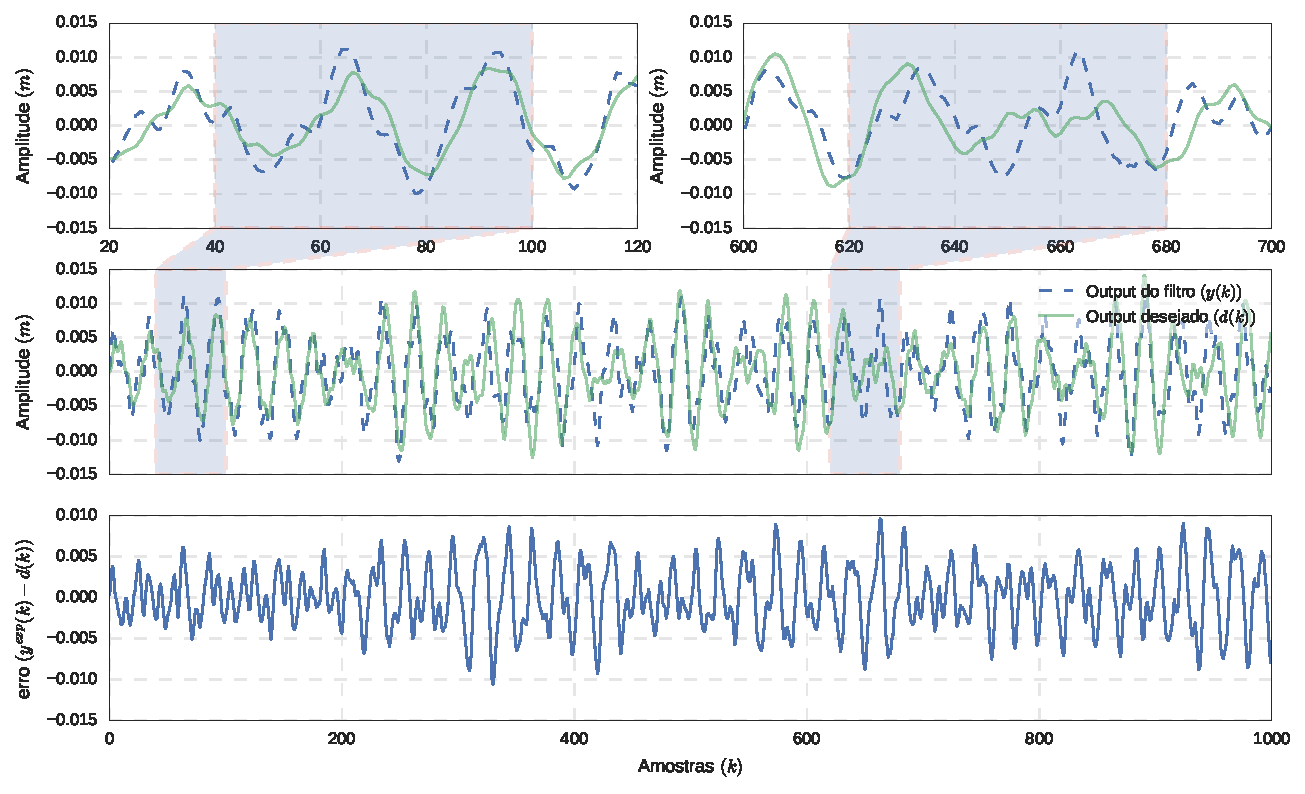
\includegraphics[scale=0.7]{F1_1000_10_mu_002_pred}
	\caption{Predição do filtro obtido com $ F=F_1 $, $ N=1000 $ e $ SNR=10 $.}
	\label{fig:F1_1000_10_mu_002_pred}
\end{figure}

\section{Resultados para $ F_2 $}
\subsection{Adaptação do filtro}

Os resultados da adaptação do filtro para uma força $ F_2 $ (ruído branco) com $ N=1000 $ são mostrados na \cref{fig:F2_1000_90_conv}, \cref{fig:F2_1000_50_conv} e \cref{fig:F2_1000_10_conv} para $ SNR = $ 90, 50 e 10  respectivamente. Neste caso, mesmo com o filtro possuindo 8 vezes mais coeficientes ($ Nc = $ 800), não foi possível obter a convergência.

A convergência só pode ser obtida para uma amostragem com $ N= $ 5000 e um filtro com 1800 coeficientes. Os resultados da adaptação para $ N= $ 5000 são mostrados na \cref{fig:F2_5000_90_conv}, \cref{fig:F2_5000_50_conv} e \cref{fig:F2_5000_10_conv} para $ SNR = $ 90, 50 e 10  respectivamente. Podemos observar que, mesmo para um nível de ruído elevado ($ SNR=10 $) o filtro apresentou uma boa convergência após aproximadamente 1600 iterações.

\begin{figure}
	\centering
	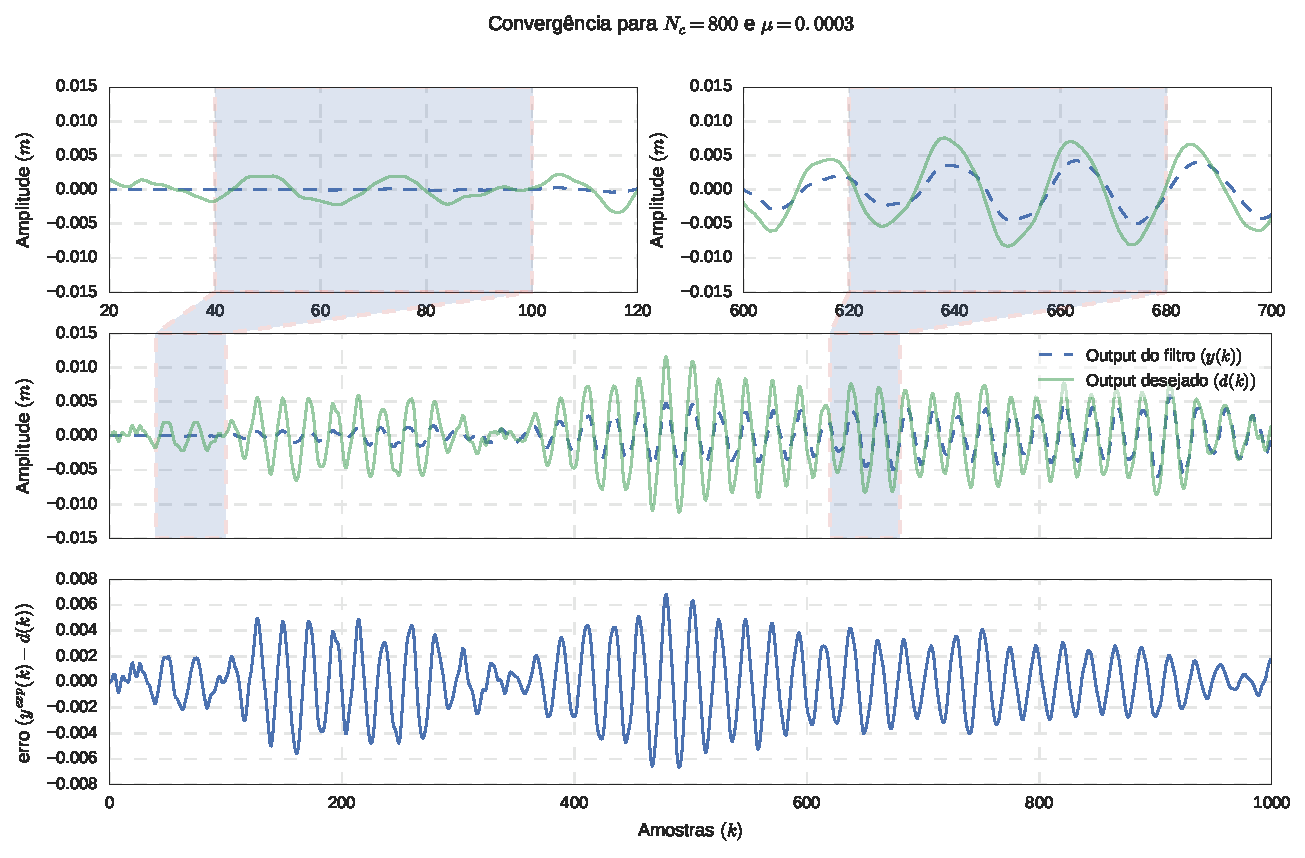
\includegraphics[scale=0.7]{F2_1000_90_conv}
	\caption{Evolução do filtro para $ F=F_2 $, $ N=1000 $ e $ SNR=90 $.}
	\label{fig:F2_1000_90_conv}
\end{figure}

\begin{figure}
	\centering
	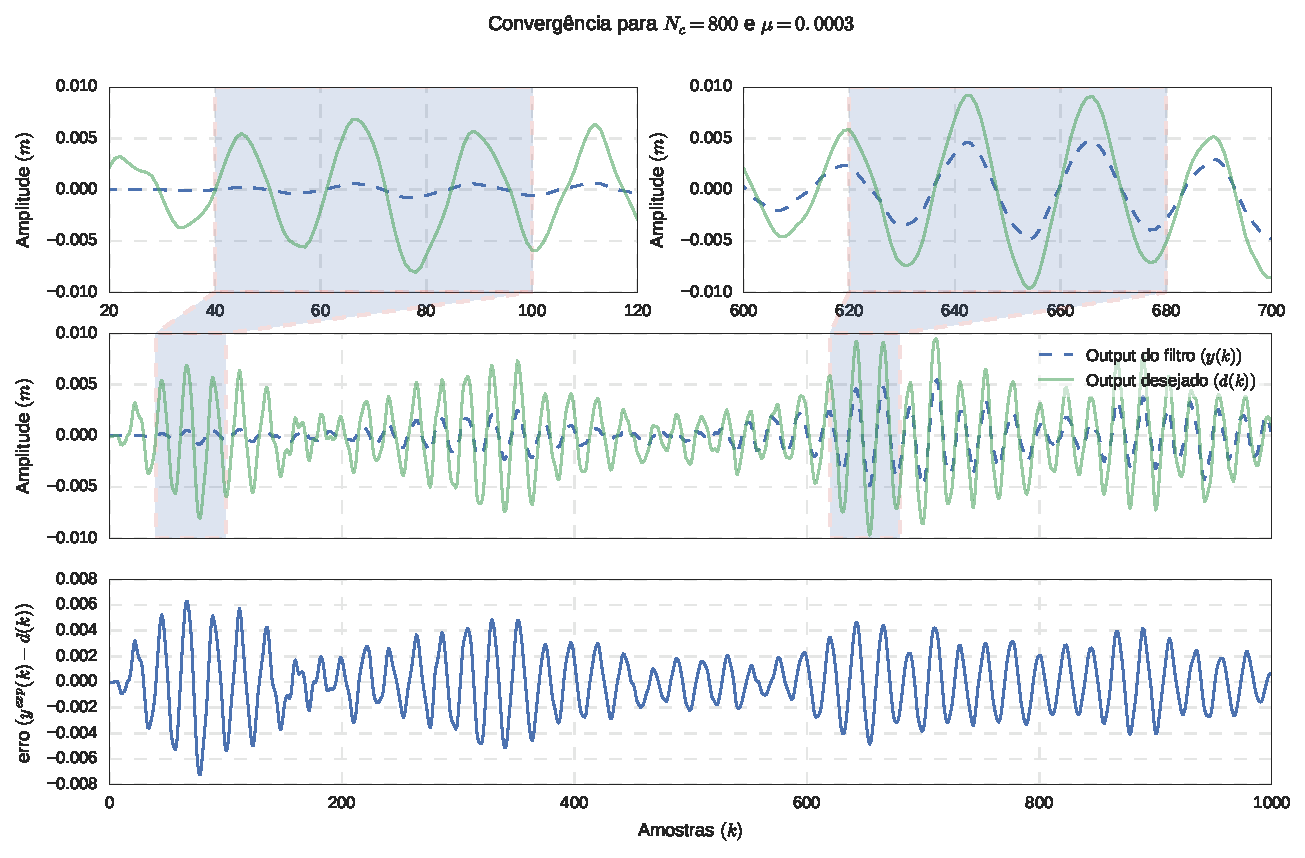
\includegraphics[scale=0.7]{F2_1000_50_conv}
	\caption{Evolução do filtro para $ F=F_2 $, $ N=1000 $ e $ SNR=50 $.}
	\label{fig:F2_1000_50_conv}
\end{figure}

\begin{figure}
	\centering
	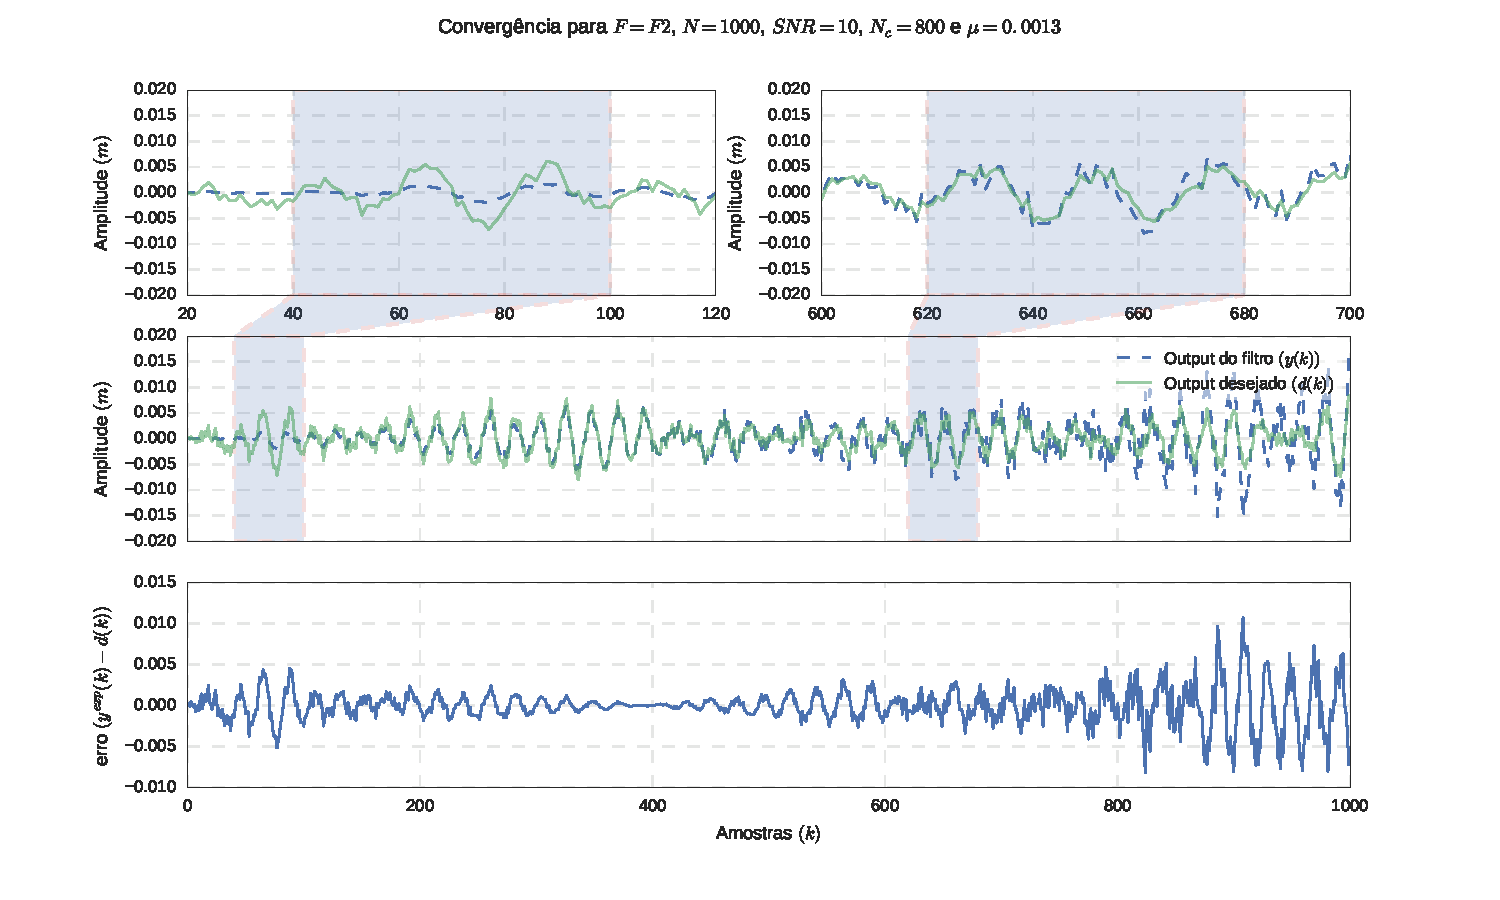
\includegraphics[scale=0.7]{F2_1000_10_conv}
	\caption{Evolução do filtro para $ F=F_2 $, $ N=1000 $ e $ SNR=10 $.}
	\label{fig:F2_1000_10_conv}
\end{figure}

\begin{figure}
	\centering
	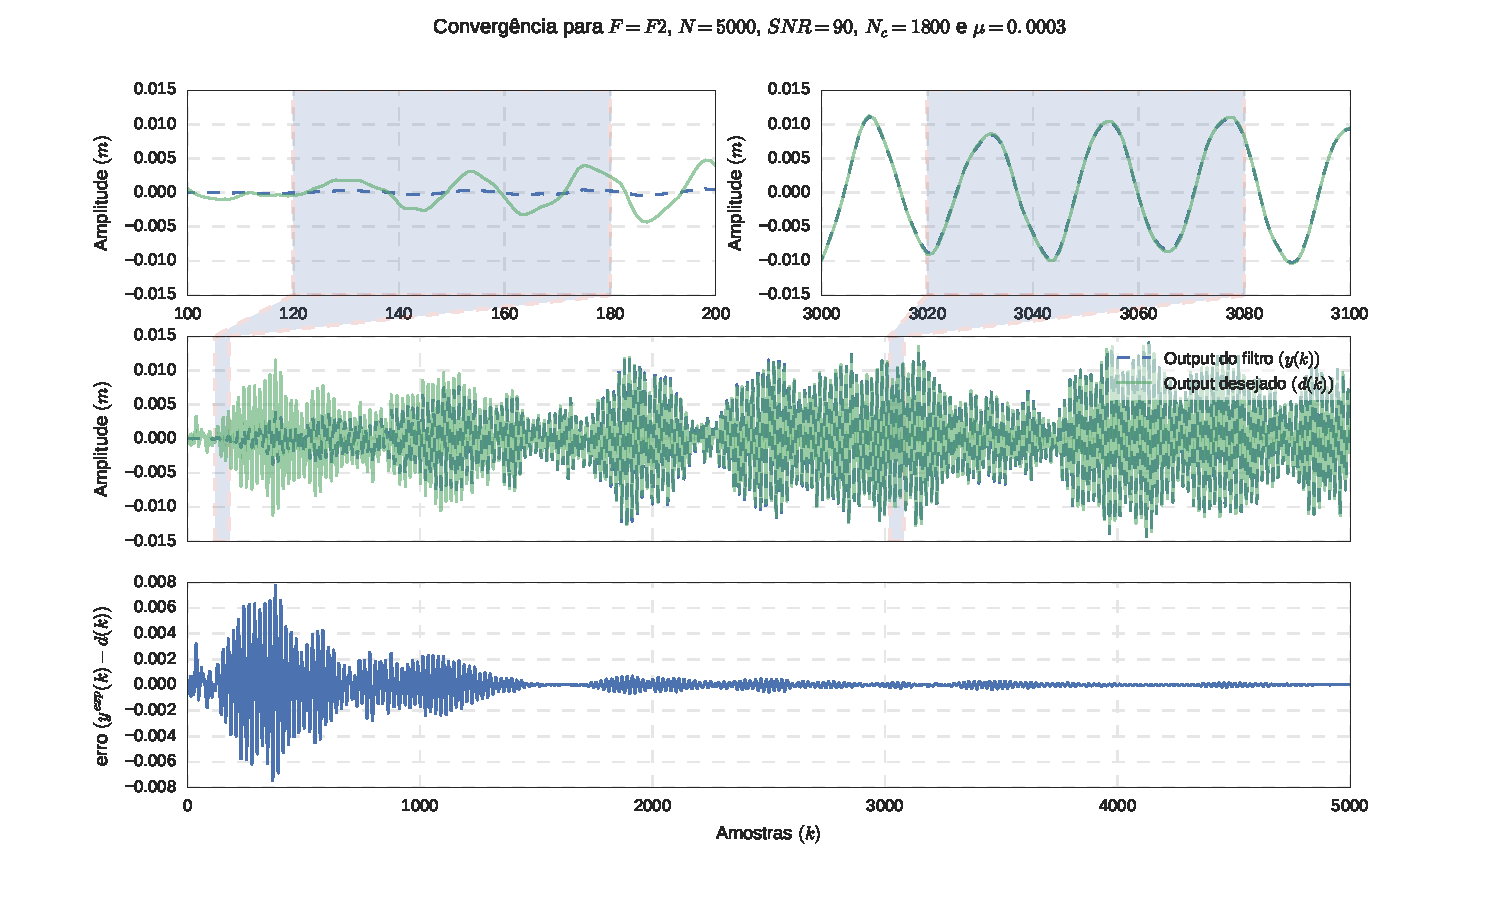
\includegraphics[scale=0.7]{F2_5000_90_conv}
	\caption{Evolução do filtro para $ F=F_2 $, $ N=5000 $ e $ SNR=90 $.}
	\label{fig:F2_5000_90_conv}
\end{figure}

\begin{figure}
	\centering
	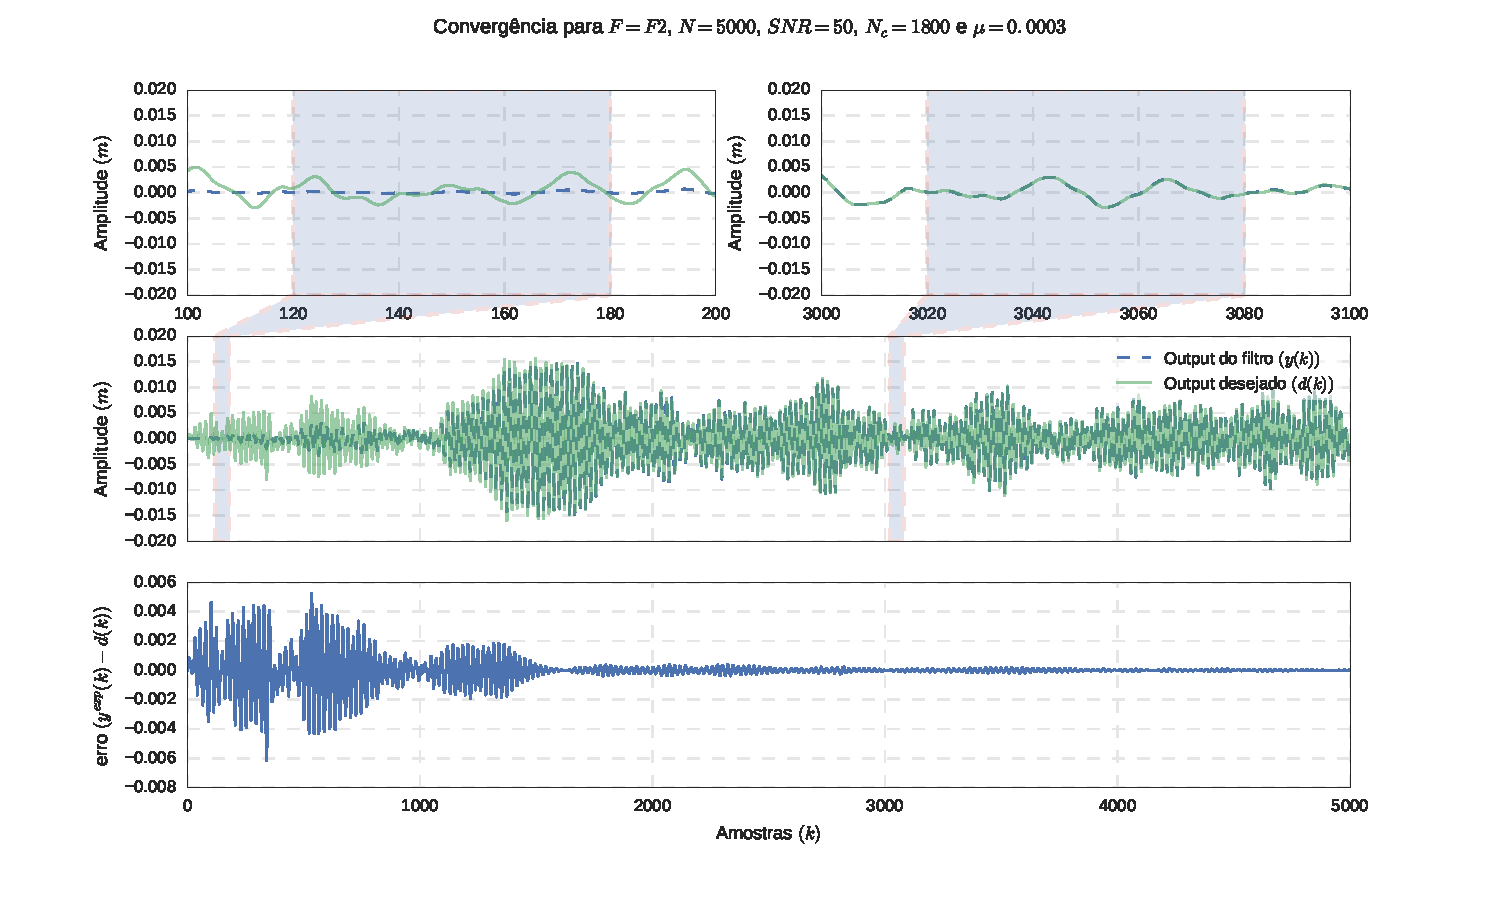
\includegraphics[scale=0.7]{F2_5000_50_conv}
	\caption{Evolução do filtro para $ F=F_2 $, $ N=5000 $ e $ SNR=50 $.}
	\label{fig:F2_5000_50_conv}
\end{figure}

\begin{figure}
	\centering
	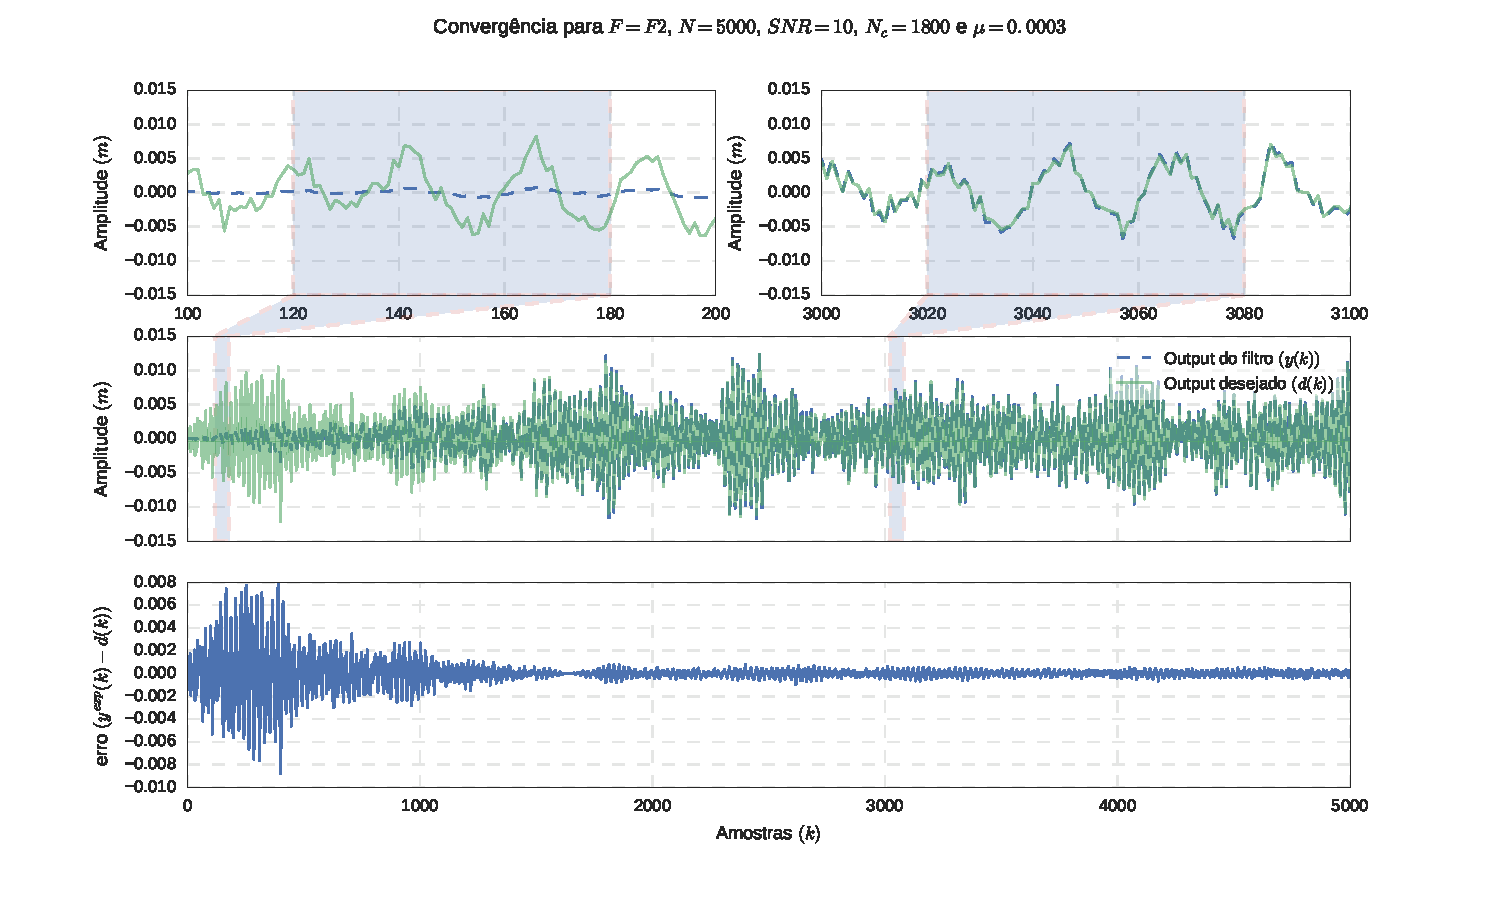
\includegraphics[scale=0.7]{F2_5000_10_conv}
	\caption{Evolução do filtro para $ F=F_2 $, $ N=5000 $ e $ SNR=10 $.}
	\label{fig:F2_5000_10_conv}
\end{figure}

\subsection{FRF do filtro}
Para a análise das FRFs iremos utilizar os filtros obtidos com $ N=5000 $, já que apenas estes apresentaram convergência nos seus coeficientes. Além disso, assim como na análise de $ F_1 $, apenas as FRFs do último vetor de coeficientes do filtro serão apresentadas.

\begin{figure}
	\centering
	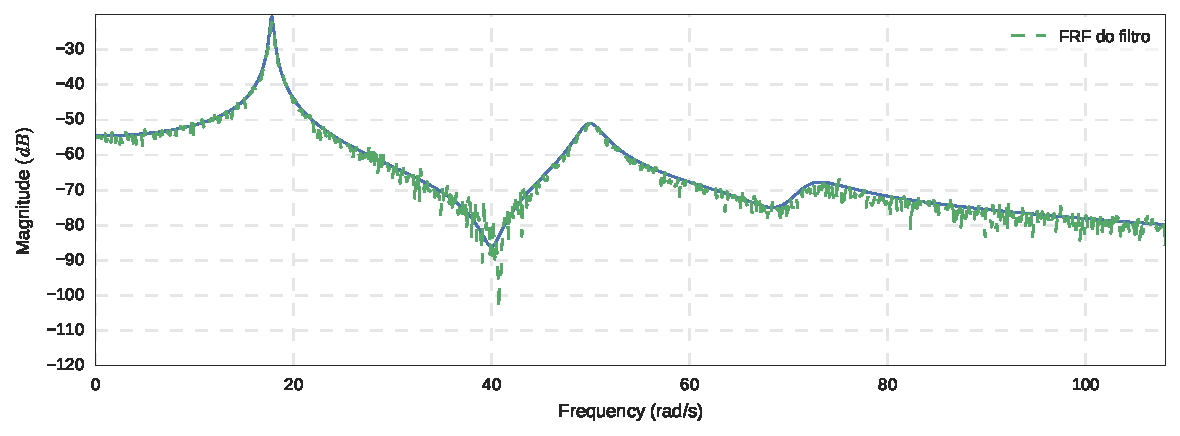
\includegraphics[scale=0.7]{F2_5000_90_FRF_med_False}
	\caption{FRF do filtro obtido para $ F=F_2 $, $ N=5000 $ e $ SNR=90 $.}
	\label{fig:F2_5000_90_FRF_med_False}
\end{figure}

A \cref{fig:F2_5000_90_FRF_med_False} mostra que para $ SNR=90 $ a FRF do filtro apresenta excelentes resultados quando comparada à FRF real do sistema. Os três picos referente às frequências naturas foram capturados, além disso a queda na amplitude devido o fenômeno de anti-ressonância também é claramente observado. Outro ponto importante é que, mesmo nas frequências mais elevadas e distantes das frequências naturais, a FRF do filtro reproduziu com exatidão os valores de amplitude esperados.

\begin{figure}
	\centering
	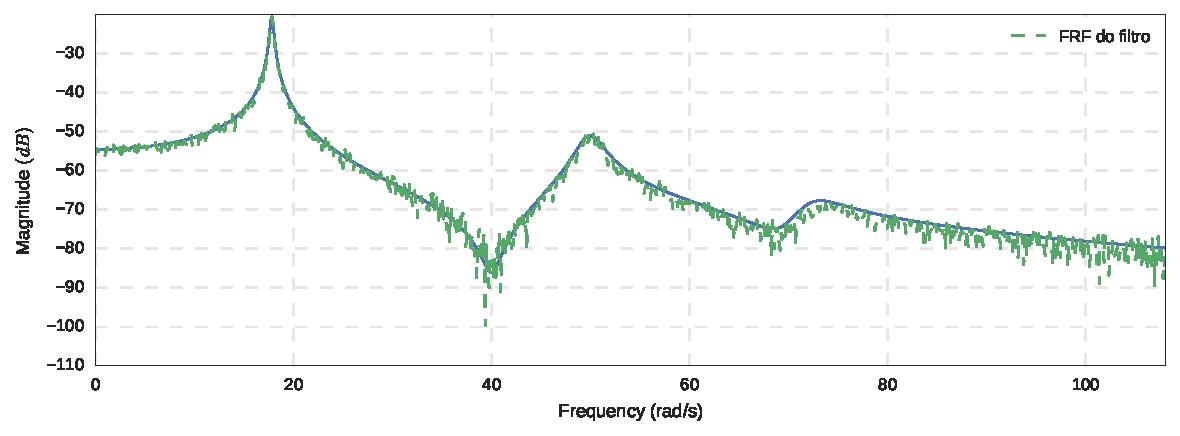
\includegraphics[scale=0.7]{F2_5000_50_FRF_med_False}
	\caption{FRF do filtro obtido para $ F=F_2 $, $ N=5000 $ e $ SNR=50 $.}
	\label{fig:F2_5000_50_FRF_med_False}
\end{figure}

A \cref{fig:F2_5000_50_FRF_med_False} mostra que, para $ SNR=50 $, os resultados ainda são satisfatórios. No entanto, ao aumentarmos o nível de ruído no sinal, podemos notar que para frequências mais elevadas a FRF do filtro apresenta uma maior variação, diferindo um pouco dos valores esperados quando comparamos com a FRF do sistema.

\begin{figure}
	\centering
	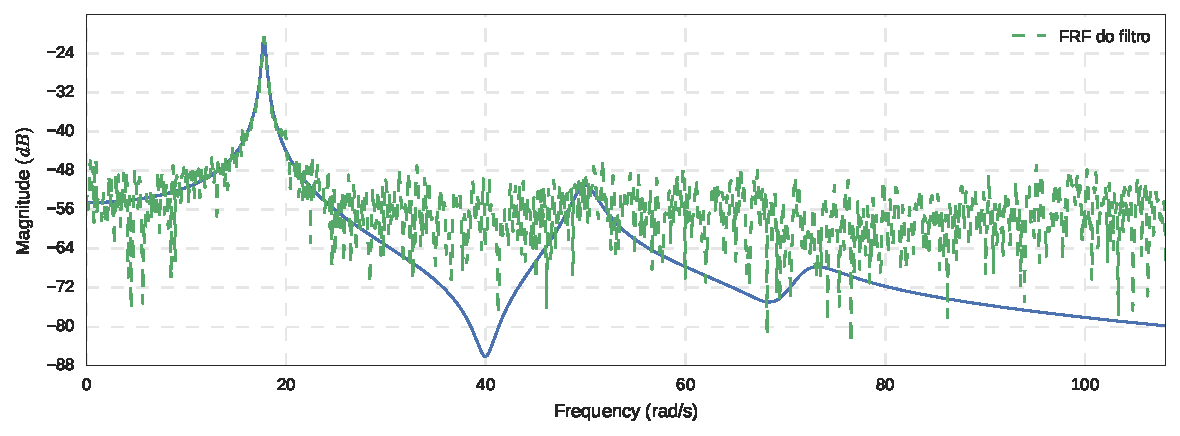
\includegraphics[scale=0.7]{F2_5000_10_FRF_med_False}
	\caption{FRF do filtro obtido para $ F=F_2 $, $ N=5000 $ e $ SNR=10 $.}
	\label{fig:F2_5000_10_FRF_med_False}
\end{figure}

A \cref{fig:F2_5000_10_FRF_med_False} apresenta a FRF para nível de ruído com $ SNR=10 $. Neste caso ainda foi possível obter um bom resultado para a primeira frequência natural, mas se afastando desse pico vemos que o filtro não descreve bem o sistema. O fenômeno de anti-ressonância não é observado e mesmo o pico referente à segunda frequência natural não pode ser visto claramente.

\subsection{Predição}

\begin{figure}
	\centering
	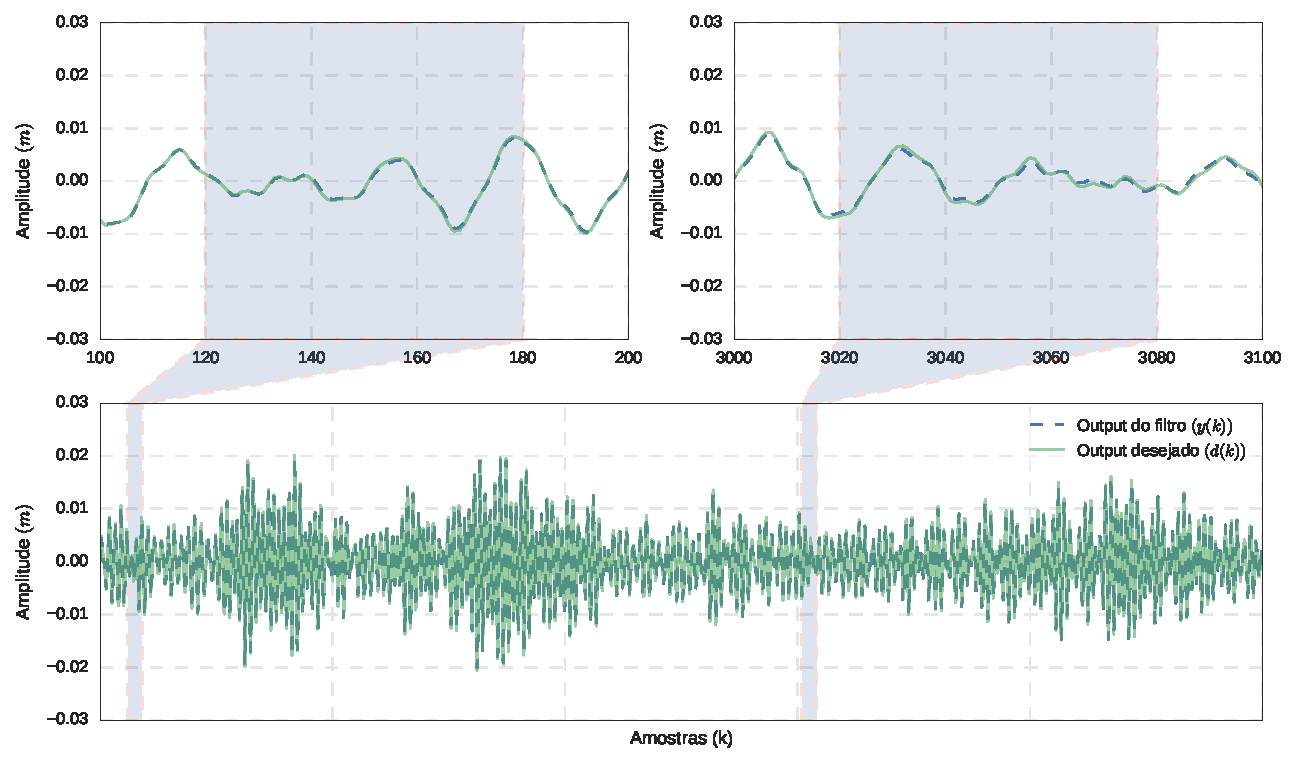
\includegraphics[scale=0.7]{F2_5000_90_pred}
	\caption{Predição do filtro obtido com $ F=F_2 $, $ N=5000 $ e $ SNR=90 $.}
	\label{fig:F2_5000_90_pred}
\end{figure}

Para a predição iremos utilizar a mesma força utilizada em $ F=F_0 $ e descrita na \ref{eq:F_3}. Os resultados da predição são apresentados na \cref{fig:F2_5000_90_pred} e na \cref{fig:F2_5000_10_pred}, para $ SNR= $ 90 e 10 respectivamente. Os resultados mostram que, para $ SNR=10 $, o filtro obtido é capaz de prever com grande exatidão a resposta do sistema.  

\begin{figure}
	\centering
	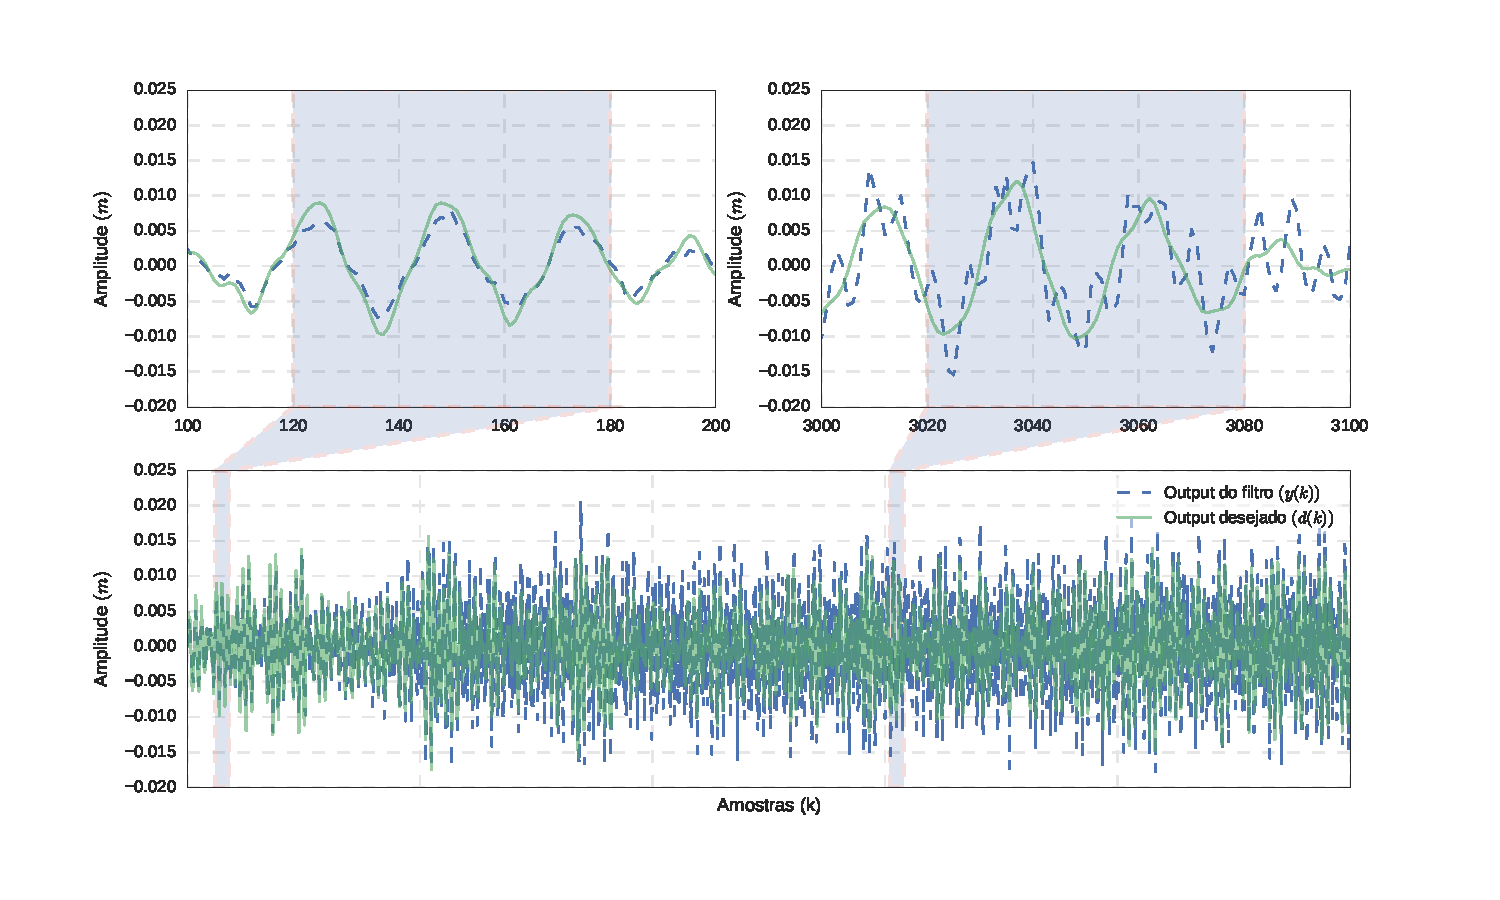
\includegraphics[scale=0.7]{F2_5000_10_pred}
	\caption{Predição do filtro obtido com $ F=F_2 $, $ N=5000 $ e $ SNR=10 $.}
	\label{fig:F2_5000_10_pred}
\end{figure}
